\section{Definição do Problema}

\begin{figure}[!h]
\caption{Descrição de problemas pelos envolvidos}
\centering % para centralizarmos a figura
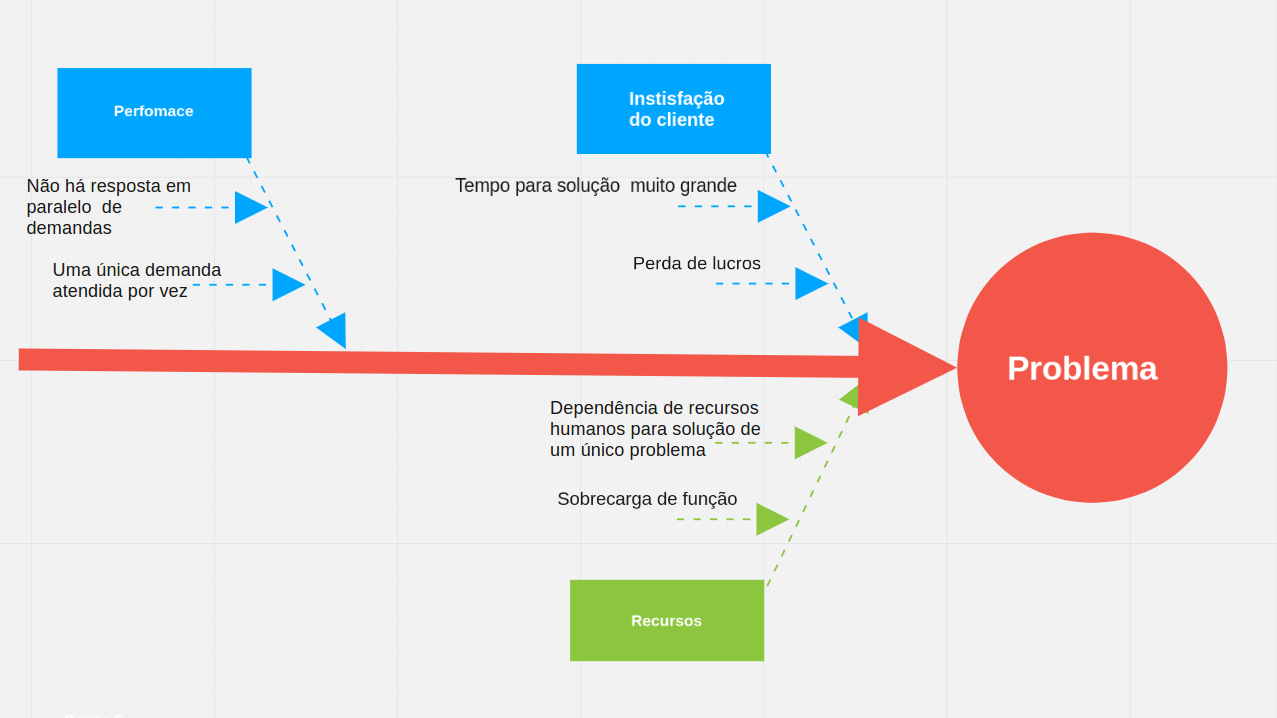
\includegraphics[width=15cm]{fishbone.png}
\label{figura:Fishbone de Problemas }
\end{figure}


\begin{itemize}[noitemsep]
  \item Problema:
    \begin{itemize}
      \item O processo de suporte ao usuário é demorado, e demanda de muitos recursos
           humanos para que seja executado.
    \end{itemize}
  \item O problema afeta:
    \begin{itemize}
      \item Os clientes
    \end{itemize}
  \item Cujo impacto é:
    \begin{itemize}
      \item	O cliente que tem a demora da solucão do seu problema
           deixa de lucrar, pois o equipamento normalmente fica sem uso.
    \end{itemize}
  \item Uma solução bem sucedida seria:
    \begin{itemize}
      \item Uma boa solução seria um conjunto de atividades, que simplifique
       automatize algumas atividades desse processo.
     \end{itemize}
\end{itemize}

\subsubsection{Objetivos}
\begin{itemize}[noitemsep]
 \item Aumentar a satifsfação do cliente
 \item Formalizar o processo atual
 \item Diminuir a necessidade de tarefas humanas no processo de suporte
 \item Diminuição do tempo de processamento de uma requisição individual
 \item Projetar e implementar a sistema de monitoramento de perfomace
 \item Encontrar gargalos
\end{itemize}

\subsubsection{Principais indicadores}
\begin{itemize}[noitemsep]
 \item Avaliação dos usuários do sistema de suporte
 \item Tempo médio gasto para a realização de um atendimento
 \item Quantidade de recurso humano gasto nesta macroatividade
\end{itemize}

\subsubsection{Envolvidos}
\begin{itemize}[noitemsep]
 \item Operador de suporte
 \item Desenvolvedor Sênior
 \item Representante de Vendas
 \item Chefe de tecnologia
\end{itemize}
